\chapter{Introduction to diagnostic medical imaging}

\section{Introduction}
In this chapter, we provide an overview of diagnostic medical imaging and its
history. Medical imaging is a field in medicine concerned with creating visual
representations of a body for the purpose of clinical analysis. Although medical
imaging is sometimes used for non-diagnostic purposes, we will only concern
ourselves with diagnostic medical imaging. This subbranch has the goal to
facilitate diagnosis of medical conditions without the need for invasive
procedures. Over the past fifty years, this discipline has matured
significantly, it has become indispensible in the modern age medical setting
\cite{review}.

The most important aspect of diagnostic medical imaging is image production, but
various other aspects are involved. Image processing, image display, image
recording, image transmission and image storage are all related. Modern day
Picture Archoving and Communication Systems (PACS) provide all these features.
Once the image has been captured and processed, it can be presented to a
radiologist for diagnosis. In recent years, scientists have focussed on
augmenting the physician's diagnostic ability with various Computer Aided
Diagnosis (CAD) schemes. For example, algorithms based on machine learning are
able to autonomously detect lung nodules with ever increasing accuracy
\cite{ginneken}. Although some systems aim to make phsycians redundant in the
long term, most experts agree that software should augment them rather than
replace them entirely.

In this thesis we will \ldots %TODO focus?

In the next sections, we will discuss the history and technical background of
the most important imaging modalities.

\section{Radiography}
Radiographs are the simplest form of medical imaging based on X-rays. These rays
can travel through solid objects, but attenuate based on the materials they met
along their path. For example, when passing through a human hand, the
attenuation is stronger when passing through bones rather than through soft
tissue. The image can be recorded (in negative) on ordinary photographic paper
and processed in darkrooms. \autoref{fig:xrayhand} shows the result.

\begin{figure}[ht]
\begin{center}
  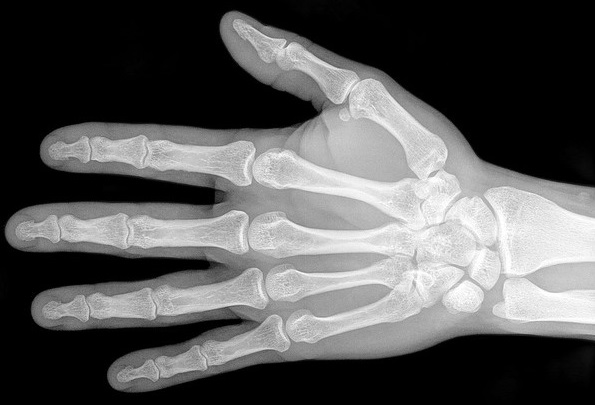
\includegraphics[width=\linewidth]{img/xrayhand.jpg}
  \caption{X-ray image of a human hand. In this negative image, bones are
  lighter because fewer X-rays managed to get through them.}
  \label{fig:xrayhand}
\end{center}
\end{figure}

\subsection{History}
Radiography - and indeed many other imaging modalities - build on the work of
Wilhelm Konrad R\"ontgen, a German physicist who produced and detected X-rays
for the first time on 8 November 1895. These X-rays (X for unknown) had the
remarkable property of being attenuated at different rates when passing through
various materials. For example, bone strongly attenuates the X-rays while soft
tissue does much less so. R\"ontgen also discovered that the radiation can be
captured on a photographic plate, just like regular light. He presented his
findings in his paper ``On a new kind or rays'' \cite{rontgen}. This discovery
earned him the Nobel Prize in Physics in 1901.

Only two weeks after his discovery he produced the first X-ray photo of his
wife's hand, after which she reportedly exclaimed: ``I have seen my death!''.
Just a couple of months later, X-rays were already being used in a clinical
setting on patients.

\subsection{Technical background}
To better understand the internal workings of imaging devices, we present a
simplified mathematical and physical background based on the book of prof.
Suetens\cite{suetens}. X-rays are simply a form of electromagnetic waves
consisting of photons with a wavelength $\lambda$ on the order of Angstr\o ms
($10^{-10}$m). The corresponding frequency $f$ places these rays firmly in the
ionizing (radioactive) part of the spectrum. The energy of such a wave can be
calculated with the following formula, where $c$ is the speed of light and $h$
is Planck's constant.

\begin{equation}
	E = hf = \frac{hc}{\lambda}.
\end{equation}

X-rays are generated in an X-ray tube, a vacuum tube consisting of a cathode and
an anode current flowing through the cathode releases electrons,
which are accelerated toward the anode by an applied voltage. Once the electrons
hit the anode, they release part of their energy in the form of X-ray photons.
Thus, the two most important settings of an X-ray scan are the applied
current multiplied by the exposure time (mA $\cdot$ s) and the applied voltage
(keV).

The attenuation of X-rays through materials can easily be modeled using an
attenuation coefficient $\mu$. The beam intensity when passed through a
homogeneous material of depth $d$ is given by: 

\begin{equation}
	I_{out} = I_{in} e^{-\mu d}.
\end{equation}

To capture X-rays, a detector is needed. Traditionally, a screen-film detector
was used. The familiar photographic film alone is very inefficient
at capturing X-rays: only about 2\% of all photons are absorped. Because X-rays
are radioactive, the applied dose cannot simply be increased to improve the
image quality. Instead, an intensifier screen is used in front of the film. This
screen contains heavy chemical elements, whose electrons are excited by the
incoming photons. When returning to their original state, these electrons emit
more photons that can be captured by the film, raising the absorption efficiency
to about 50\%.

%TODO mammo

\subsection{Recent advancements}
Relatively recently, X-ray systems have moved away from analogue detectors
towards digital ones. Much like digital photographs, digital X-ray scans are far
easier to store, copy, post-process and share. On top of that, they typically
have a much wider exposure range making them more tolerant to over- and
underexposure. These detector systems use storage phosphors to temporarily hold
the absorped radiation instead of immediately releasing it in the form of
photons. This phenomenon is caused by electron traps in the doped material.
Later, this phophor can be read out pixel-wise using an optical detector array
and a laser that gives the eletrons enough energy to escape their trap. The main
obstacle for this paradigm shift was the large pixel size. Pixels of 1 mm make
it much more difficult for a radiologist to analyze the image in its digital
form. Only by the time pixels could be as small as 0.1 mm did the medical world
embrace digital detectors \cite{review}.

Even newer devices use active matrix flat panel detectors. These detectors are
able to produce near real time images where storage phosphors and older
technlogies required minutes or more of processing time. %TODO how?

\subsubsection{A note on digital image quality}
The quality of a digital image can be expressed in three dimensions: resolution,
contrast and noise \cite{suetens}.

Resolution is sometimes simply stated as the pixel density (dots per inch).
However, this only provides an upper bound because in practise neighbouring
pixels can be correlated. For example, due to the imperfect nature of the
recording equipment, a single point can appear as blurred blob on the resulting
image. This blob is called the Point Spread Function (PSF), and is a better
measure for the actual image resolution. If the resolution is isotropic, the
Line Spread Function (LSF) - measured in distinguishable line pairs per mm
(lp/mm) - can also be used. Alternatively, the Optical Transfer Function (OTF,
sometimes also MTF) representing amplitude and phase shifts of a sinusoidal
target can be used. In fact, this OTF is nothing more than the Fourier transform
of the PSF or LSF.

Second, contrast is the intensity difference between neighbouring regions of the
image. More formally, contrast at a given frequency is the amplitude component
of the image at that frequency in the frequency domain (calculated using the
Fourier transform). Contrast is dependent on the whole imaging process, but also
on the size and shape of the objects in the image.

Third, noise is partly the result of interfering processes. Yet, it is also
inherent to the electromagnetic radiation itself because the waves themselves
are stochastic processes. An important measure is the Signal to Noise Ratio
(SNR) or more appropriately Contrast to Noise Ratio (CNR). Noise can be
estimated by examining the result of an scan with no object present, a so-called
flat-field image. Another measure for the amount of noise is the Wiener
spectrum.

In addition to these three elements, sometimes artefacts appear on scans. The
causes of these artificial image features vary widely depending on the image
modality used and can also be caused by excessive post-processing.

\subsection{Future expectations}
Ever since CT and MRI scanners made their way into hospitals, they have taken
over many of the tasks traditionally reserved for basic radiography. This
declining trend is expected to continue in the foreseeable future.

\section{X-ray computed tomography}
One step up from basic radiography is computed tomography (Greek for ``slice
writing''). The goal here is to create image slices of patients in the
cross-sectional plane rather than the frontal plane. To accomplish this, the X-ray
source-detector pair is rotated around the patient. From this raw data, a
so-called filtered back projection algorithm can reconstruct the whole cross
section image. A computer is needed to make sense of the output, hence the
\emph{computed} in the name. \autoref{fig:ctscan} shows an example of a chest
CT scan.

\begin{figure}[ht]
\begin{center}
  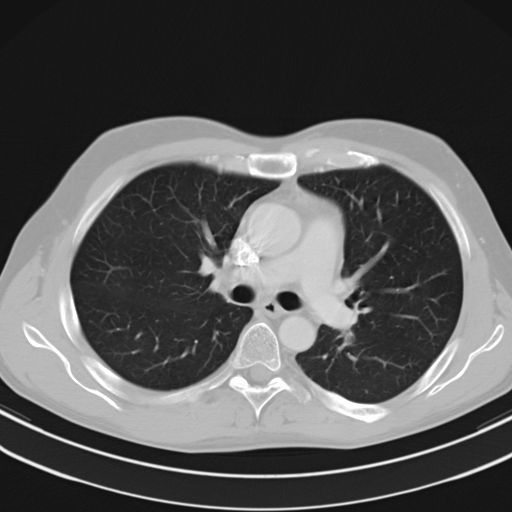
\includegraphics[width=0.4\linewidth]{img/ct-thorax.jpg}
  \caption{Example of a thoracic CT scan. The heart is clearly visible in the
  center. Bones (ribs, sternum, spine) are also easy to spot in the periphery.
  The large black area represents the lungs filled with air.}
  \label{fig:ctscan}
\end{center}
\end{figure}

\subsection{History}
Before computed tomography became possible, some simpler techniques were already
being used to obtain slices from inside the patient's body. These techniques
were simply called (non-computed) tomography. One example is linear tomography,
where source and detector move on parallel tracks, but in opposite directions,
during the scanning process. This way, one section of the patient is always
projected on the same spot of the detector, while the rest is averaged out.
Obviously, these techniques where nowhere near as accurate as the CT scanners we
know today.

In 1917, Johann Radon - an Austrian mathematician - presented the first
algorithm to reconstruct a function from its projections: the Radon transform
\cite{radon}.

In the 1960's, the South African Allan McLeod Cormack continued working on the
mathematics invented by Radon. A decade later, in 1972, the first operational
brain CT scanner (the EMI scanner) was designed by Godfrey Hounsfield, an
Englishman. A scan took about 5 minutes, after which a computer performed
calculation for up to 150 minutes. The final output was a 80px $\times$ 80px
image. Cormack and Hounsfield shared the 1979 Nobel Prize in Physiology and
Medicine for their work related to CT scans.

%helical, 1989
%multislice, 1998

\begin{figure}[ht]
\begin{center}
  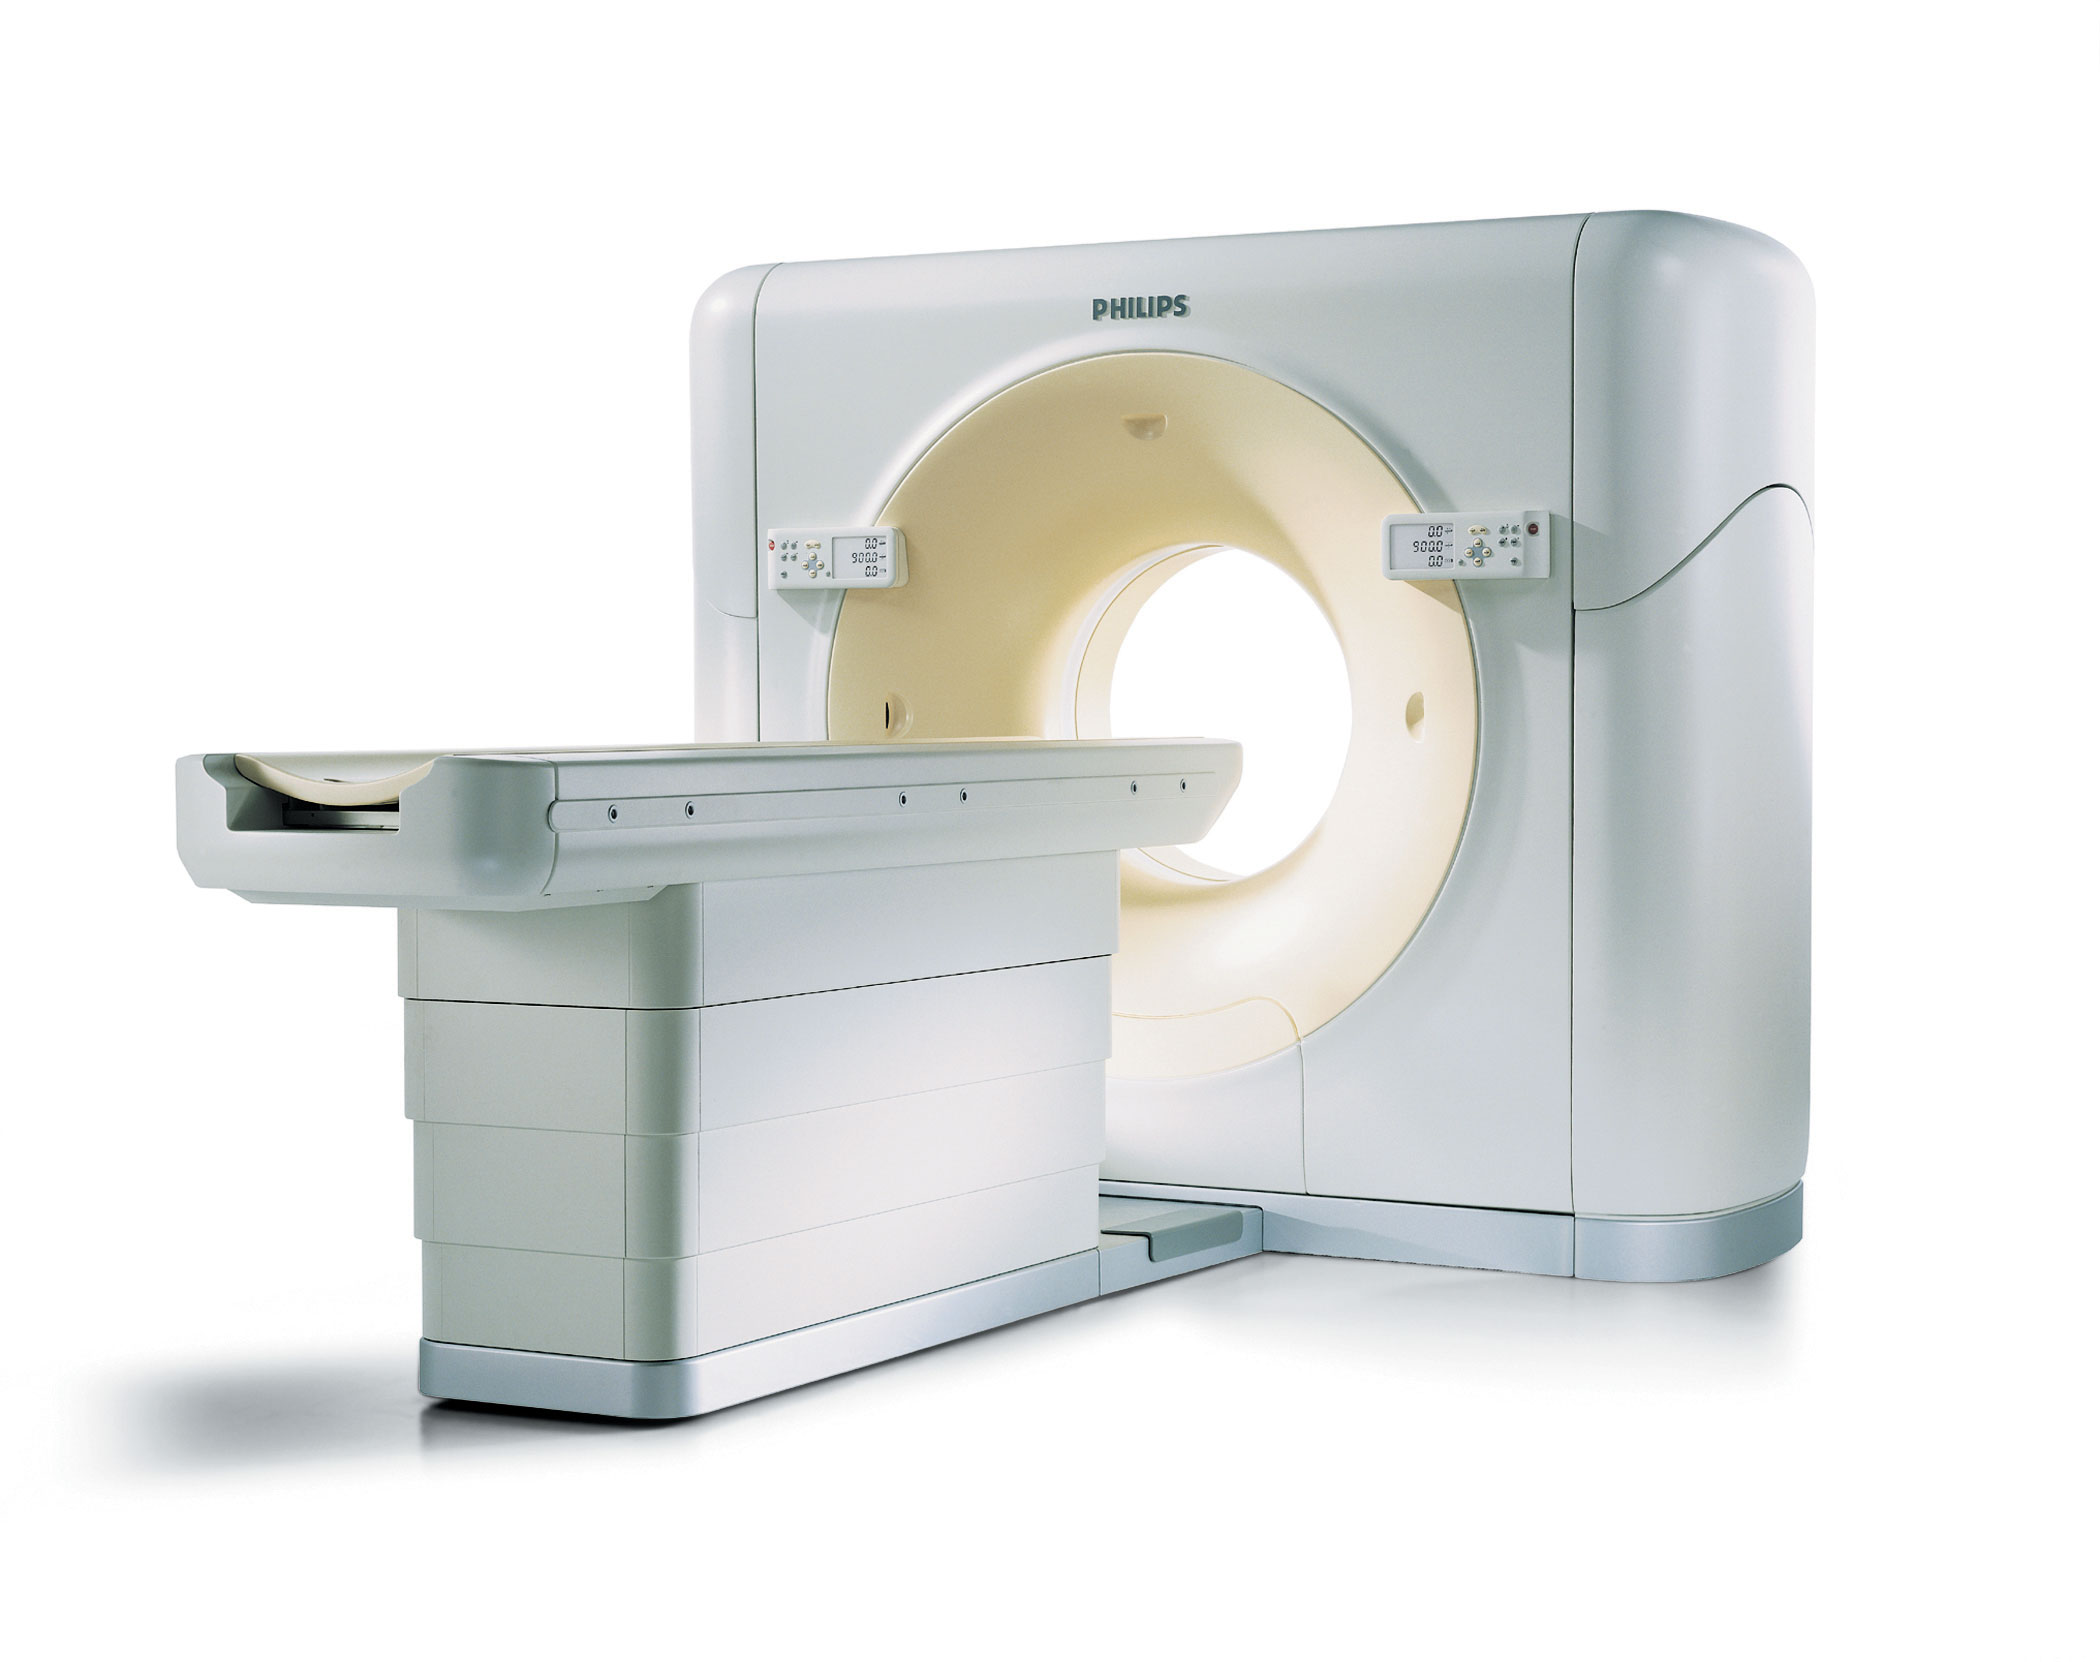
\includegraphics[width=\linewidth]{img/ctscanner.jpg}
  \caption{A CT scanner made by Philips. The patient takes place on the table
  and slowly slides through the toroid wherein the rotating X-ray
  source-detector pair is embedded.}
  \label{fig:ctscanner}
\end{center}
\end{figure}

\subsection{Technical background}
Just like radiographs, CT scanners are based on X-ray technology. They also
require a source and a detector, but this time they can rotate along the
patient. For every rotation angle $\theta$, we obtain an intensity profile
$I_\theta(r)$ along the axis $r$ perpendicular to the incoming X-rays (with
uniform intensity $I_0$). The family of functions $I_\theta$ can be transformed
into an attenuation profile $p(r, \theta) = -\ln \tfrac{I_\theta(r)}{I_0}$
(often called a sinogram). This $p(r, \theta)$ is called the Radon transform of
the attenuation distribution $\mu(x,y)$ in the slice plane.
\begin{equation}
	p(r, \theta) = \mathscr{R}\{ \mu(x,y) \}
\end{equation}

In short, the projections $p$ is what we can measure (or at least sample at
fixed intervals) and the attentuation distribution $\mu$ is what we are
interested in. The maths required to go from the latter to the former are pretty
straightforward, but the reverse is more complicated. The inverse Radon
transform $\mu = \mathscr{R}^{-1}(p)$ is needed.

We will not go into details, but the solution lies in the projection theorem.
This theorem states that the 2D Fourier transform $M(k_x, k_y)$ of $\mu(x,y)$
is equal to the 1D Fourier transform $P(k, \theta)$ of $p(r, \theta)$ (save for
a simple polar coordinate transformation).

\begin{equation}
P(k, \theta) = M(k \cos \theta, k \sin \theta)
\end{equation}

Because the inverse Fourier transform is well understood, we have a solution to
our problem. Simple calculate $P$ from $p$ as explained above, and then apply
the inverse 2D Fourier transform to obtain $\mu$. By using the polar version of
the Fourier transform, we can reduce artifacts. This approach is called filtered
back projection \cite{suetens}.

After all the calulcations are performed, we typically acquire a 512px $times$
512px scan. The values of the pixels in a CT scan are referred to as the CT
numbers and are expressed in Hounsfield Units (HU). They are calculated using
the fomula below, where $\mu$ is again the attenuation coefficient.
\begin{equation}
	\text{CT number} = \frac{\mu -
	\mu_{\text{H}_2\text{O}}}{\mu_{\text{H}_2\text{O}}} \cdot 1000
\end{equation}

From this, it becomes obvious that the CT number of air (with $\mu = 0$) is
-1000 HU and that the CT number of water is 0 HU. Bones on the other hand have a
very high attenuation coefficient and thus have a CT number in the thousands.
Soft tissue lies somewhere in between.

\subsection{Recent advancements}
The previous section assumed parallel X-ray beams. However, newer generation
scanners often employ cone-shaped beams. The procedure outlined above can
reconstruct a single slice by rotating around the subject by 180 degrees at a
time (a circular CT). On the other hand, modern CT scanners often spiral around
the patient while he moves through the toroid (a helical CT) to speed up the
process and thus lowering the exposure. Another useful trick is to capture
multiple slices at once by using multiple detector arrays. Until recently,
manufactureres were in a so-called \emph{slice wars} to offer the most detector
arrays. Needless to say, all this substantially complicates the maths to perform
a back projection, but it is still possible and in fact often used today.

Another point of interest today is the combination of successive CT slices to
generate a 3D model of the patient. Because of advancements in computer
technology and algorithms, we can now post-process this 3D model to
automatically segment the bones and organs. This can for example help physicians
plan their actions before and during complex surgery. %TODO cite

\subsection{Future expectations}
Because CT scanners still require relatively high doses of radiation, this is
not an ideal solution. MRI scanners offer a safer alternative, but the large
magnetic fields produced make them impossible to use on patients with certain
implants. Another advantage over MRI is the superior sub-millimeter resolution
that only CT scans can handle. These are only some of the reasons why they will
not be replaced anytime soon. Future research will attempt to make CT scanners
even faster and allow them to produce clear images (high contrast) with lower
doses.

\section{Magnetic resonance imaging}

\subsection{History}

\subsection{Technical background}

\subsection{Recent advancements}

\subsection{Future expectations}

\section{Nuclear medicine imaging}

\subsection{History}

\subsection{Technical background}

\subsection{Recent advancements}

\subsection{Future expectations}

%ultrasound, img processing, automated diagnosis

%ROC
